\documentclass[]{article}
\usepackage{lmodern}
\usepackage{amssymb,amsmath}
\usepackage{ifxetex,ifluatex}
\usepackage{fixltx2e} % provides \textsubscript
\ifnum 0\ifxetex 1\fi\ifluatex 1\fi=0 % if pdftex
  \usepackage[T1]{fontenc}
  \usepackage[utf8]{inputenc}
\else % if luatex or xelatex
  \ifxetex
    \usepackage{mathspec}
    \usepackage{xltxtra,xunicode}
  \else
    \usepackage{fontspec}
  \fi
  \defaultfontfeatures{Mapping=tex-text,Scale=MatchLowercase}
  \newcommand{\euro}{€}
\fi
% use upquote if available, for straight quotes in verbatim environments
\IfFileExists{upquote.sty}{\usepackage{upquote}}{}
% use microtype if available
\IfFileExists{microtype.sty}{%
\usepackage{microtype}
\UseMicrotypeSet[protrusion]{basicmath} % disable protrusion for tt fonts
}{}
\usepackage[margin=1in]{geometry}
\usepackage{longtable,booktabs}
\usepackage{graphicx}
\makeatletter
\def\maxwidth{\ifdim\Gin@nat@width>\linewidth\linewidth\else\Gin@nat@width\fi}
\def\maxheight{\ifdim\Gin@nat@height>\textheight\textheight\else\Gin@nat@height\fi}
\makeatother
% Scale images if necessary, so that they will not overflow the page
% margins by default, and it is still possible to overwrite the defaults
% using explicit options in \includegraphics[width, height, ...]{}
\setkeys{Gin}{width=\maxwidth,height=\maxheight,keepaspectratio}
\ifxetex
  \usepackage[setpagesize=false, % page size defined by xetex
              unicode=false, % unicode breaks when used with xetex
              xetex]{hyperref}
\else
  \usepackage[unicode=true]{hyperref}
\fi
\hypersetup{breaklinks=true,
            bookmarks=true,
            pdfauthor={},
            pdftitle={4\^{}\{th\} Report},
            colorlinks=true,
            citecolor=blue,
            urlcolor=blue,
            linkcolor=magenta,
            pdfborder={0 0 0}}
\urlstyle{same}  % don't use monospace font for urls
\setlength{\parindent}{0pt}
\setlength{\parskip}{6pt plus 2pt minus 1pt}
\setlength{\emergencystretch}{3em}  % prevent overfull lines
\setcounter{secnumdepth}{5}

%%% Use protect on footnotes to avoid problems with footnotes in titles
\let\rmarkdownfootnote\footnote%
\def\footnote{\protect\rmarkdownfootnote}

%%% Change title format to be more compact
\usepackage{titling}

% Create subtitle command for use in maketitle
\newcommand{\subtitle}[1]{
  \posttitle{
    \begin{center}\large#1\end{center}
    }
}

\setlength{\droptitle}{-2em}
  \title{\(4^{th}\) Report}
  \pretitle{\vspace{\droptitle}\centering\huge}
  \posttitle{\par}
  \author{}
  \preauthor{}\postauthor{}
  \predate{\centering\large\emph}
  \postdate{\par}
  \date{2/2/2016}



\begin{document}

\maketitle


\section{Introduction}

\ldots{}

\section{Framework}

The algorithm has two main parts

\begin{itemize}
    \item Simulate Data
    \item Estimate parameters
\end{itemize}

\section{Models}

\[ \lambda = f(traits) \] \[ \mu = f(traits) \]

\begin{itemize}

    \item[Model 1:]
        $$\lambda_i = e^{\theta_0 + \theta_1 a_i} $$
        $$ \mu_i = e^{\varphi_0 + \varphi_1 a_i} $$
    \item[Model 2:] 
        $$\lambda_i = \theta_0 + \theta_1 a_i $$
        $$ \mu_i = \varphi_0 + \varphi_1 a_i $$
    \item[Model 3:]
        $$\lambda_i = \frac{\theta_0}{1+e^{-\theta_1 a_i}}$$
\end{itemize}

\subsection{Questions:}

\begin{itemize}
        \item Are those models realistic?, there is any bilogical meaning on this models? 
        \item Would be a non-parametric approach a better alternative of those models?

    \end{itemize}

\section{Estimations}

\% latex table generated in R 3.2.1 by xtable 1.8-0 package \% Fri Jan
29 20:13:13 2016

\begin{table}[ht]
\centering
\begin{tabular}{rrrrrrr}
  \hline
 & n & real value & mean & median & min & max \\ 
  \hline
1 & 1000 & 3.00 & 3.00 & 2.98 & 0.62 & 5.81 \\ 
  2 & 1000 & 4.00 & 5.03 & 3.95 & -591.87 & 2410.71 \\ 
  3 & 1000 & 1.00 & 1.56 & 0.87 & -13.42 & 347.45 \\ 
  4 & 1000 & 2.00 & -1.03 & 1.63 & -4045.67 & 2003.04 \\ 
   \hline
\end{tabular}
\caption{Model 1}
\end{table}

\begin{table}[ht]
\centering
\begin{tabular}{rrrrrrr}
  \hline
 & n & real value & mean & median & min & max \\ 
  \hline
1 & 1000 & 3.00 & 2.83 & 2.85 & -15.46 & 17.76 \\ 
  2 & 1000 & 4.00 & 13.43 & 3.87 & -4131.72 & 3329.81 \\ 
  3 & 1000 & 1.00 & 1.02 & 0.94 & -15.02 & 18.60 \\ 
  4 & 1000 & 2.00 & -5.88 & 1.60 & -7333.90 & 3473.38 \\ 
   \hline
\end{tabular}
\caption{Model 2}
\end{table}

\begin{table}[ht]
\centering
\begin{tabular}{rrrrrrr}
  \hline
 & n & real value & mean & median & min & max \\ 
  \hline
1 & 1000.00 & 3.00 & 4.55 & 3.34 & 1.39 & 63.37 \\ 
  2 & 1000 & 4.00 & 10.09 & 2.02 & -1118.53 & 2702.20 \\ 
  3 & 1000 & 1.00 & 2.64 & 1.07 & 0.34 & 180.18 \\ 
  4 & 1000 & 2.00 & -0.75 & 1.46 & -3027.31 & 2999.15 \\ 
   \hline
\end{tabular}
\caption{Model 3}
\end{table}

\section{First section}

\subsection{A subsection}

\% latex table generated in R 3.2.1 by xtable 1.8-0 package \% Fri Jan
29 19:08:18 2016

\begin{table}[ht]
\centering
\begin{tabular}{rrrrrrr}
  \hline
 & n & real value & mean & median & min & max \\ 
  \hline
1 & 10000.00 & 3.00 & 3.02 & 3.00 & 0.02 & 6.27 \\ 
  2 & 10000.00 & 4.00 & 2.92 & 3.88 & -5344.38 & 8316.81 \\ 
  3 & 10000.00 & 1.00 & 1.30 & 0.89 & -85.51 & 1730.75 \\ 
  4 & 10000.00 & 2.00 & 0.33 & 1.41 & -14784.51 & 6445.60 \\ 
   \hline
\end{tabular}
\caption{Model 1}
\end{table}

\newpage

\section{Abstract}\label{abstract}

\emph{Lorem ipsum dolor sit amet, est ad doctus eligendi scriptorem. Mel
erat falli ut. Feugiat legendos adipisci vix at, usu at laoreet
argumentum suscipiantur. An eos adhuc aliquip scriptorem, te adhuc dolor
liberavisse sea. Ponderum vivendum te nec, id agam brute disputando
mei.}

\section{Introduction}\label{introduction-1}

Lorem ipsum dolor sit amet, est ad doctus eligendi scriptorem. Mel erat
falli ut. Feugiat legendos adipisci vix at, usu at laoreet argumentum
suscipiantur. An eos adhuc aliquip scriptorem, te adhuc dolor
liberavisse sea. Ponderum vivendum te nec, id agam brute disputando mei.

Putant numquam tacimates at eum. Aliquip torquatos ex vis, mei et quando
debitis appareat, impetus accumsan corrumpit in usu. Nam mucius facilis
singulis id, duo ei autem imperdiet instructior. Cu ceteros alienum mel,
id vix putant impedit, ex idque eruditi forensibus eum. Posse dicunt id
usu. Ei iracundia constituto sed, duo ne exerci ignota, an eum unum
conceptam.

Has audire salutandi no, ut eam dicat libris dicunt. Pri hendrerit
quaerendum adversarium ea, dicat atqui munere et sea. Illum insolens eos
ne, eu enim graece rationibus mea. At postea utamur mel, eius nonumes
percipitur at vis. Numquam similique in per, te quo saepe utroque
pericula.

Ea nonumy volumus usu, no mel inermis dissentias. Dico partiendo
vituperatoribus eum et. Mea accusam convenire te, usu populo qualisque
gloriatur ut. Eu eum oratio altera option, ad mea ignota scriptorem. Ne
suas latine vix, eos oblique sanctus pertinax cu.

\section{Methods}\label{methods}

Lorem ipsum dolor sit amet, est ad doctus eligendi scriptorem. Mel erat
falli ut. Feugiat legendos adipisci vix at, usu at laoreet argumentum
suscipiantur. An eos adhuc aliquip scriptorem, te adhuc dolor
liberavisse sea. Ponderum vivendum te nec, id agam brute disputando mei.

Putant numquam tacimates at eum. Aliquip torquatos ex vis, mei et quando
debitis appareat, impetus accumsan corrumpit in usu. Nam mucius facilis
singulis id, duo ei autem imperdiet instructior. Cu ceteros alienum mel,
id vix putant impedit, ex idque eruditi forensibus eum. Posse dicunt id
usu. Ei iracundia constituto sed, duo ne exerci ignota, an eum unum
conceptam.

\subsection{Equations}\label{equations}

The deterministic part of the model is defined by this \textbf{in-line
equation} as \(\mu_i = \beta_0 + \beta_1x\), and the stochastic part by
the \textbf{centered equation}:

\[ \frac{1}{\sqrt{2\pi}\sigma}e^{-(x-\mu_i)^2/(2\sigma^2)} \]

\subsection{Tables}\label{tables}

\begin{longtable}[c]{@{}lrrrr@{}}
\caption{This is a GLM summary table.}\tabularnewline
\toprule
& Estimate & Std. Error & t value &
Pr(\textgreater{}\textbar{}t\textbar{})\tabularnewline
\midrule
\endfirsthead
\toprule
& Estimate & Std. Error & t value &
Pr(\textgreater{}\textbar{}t\textbar{})\tabularnewline
\midrule
\endhead
(Intercept) & 0.07 & 0.11 & 0.69 & 0.49\tabularnewline
x & 1.81 & 0.11 & 17.18 & 0.00\tabularnewline
\bottomrule
\end{longtable}

\subsection{Plots}\label{plots}

\begin{figure}[htbp]
\centering
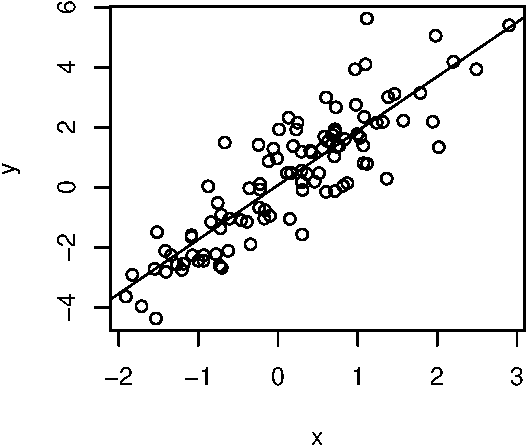
\includegraphics{rR4_files/figure-latex/carDataPlot-1.pdf}
\caption{Relationship between x and y. The solid line is least-squares
linear regression.}
\end{figure}

\end{document}
